 \documentclass[a4paper,10pt]{article}
\include{amsymb}
\include{marvosym}

\usepackage[francais]{babel}
\usepackage[cyr]{aeguill}
\usepackage[applemac]{inputenc}
\usepackage{graphicx}
\usepackage{xspace}
\usepackage[a4paper]{geometry}
\usepackage{latexsym,amsmath,amssymb,textcomp}
\usepackage{moreverb}
\usepackage{listings}
\usepackage{multirow}
\usepackage{titling}
\usepackage{mathabx}

\usepackage{pdfpages}

\usepackage{hyperref}


\newlength{\indentationnota}
\newlength{\largeurlignenota}
\newlength{\paddingnota}
\newlength{\largeurnota}
\setlength{\paddingnota}{5pt}
\setlength{\largeurnota}{0.9cm}

\definecolor{pink}{rgb}{1,0.5,1}
\makeatletter

\newenvironment{pictonote}[1]{% on passe le nom du �chier en argument
\begin{list}{}{%
\setlength{\labelsep}{0pt}%
\setlength{\rightmargin}{15pt}%
\setlength{\paddingnota}{5pt}}
\item%
\setlength{\indentationnota}{%
\@totalleftmargin+\largeurnota+\paddingnota}%
\setlength{\largeurlignenota}{%
\linewidth-\largeurnota-\paddingnota}%
\parshape=3%
\indentationnota\largeurlignenota%
\indentationnota\largeurlignenota%
\@totalleftmargin\linewidth%
\raisebox{-\largeurnota+2.2ex}[0pt][0pt]{%
\makebox[0pt][r]{%
\includegraphics[width=\largeurnota]{#1}%
\hspace{\paddingnota}}}%
\ignorespaces}{%
\end{list}}

\makeatother

\newenvironment{attention}%
{\begin{pictonote}{/Users/benjamin/Documents/Education/LaTeX/danger}}%
{\end{pictonote}}

\newenvironment{unicorn}%
{\begin{pictonote}{/Users/benjamin/Documents/Education/LaTeX/angry_unicorn}}%
{\end{pictonote}}

\newcommand\unicornbox[1]{\colorbox{pink}{\color{white}{#1}}}

\newcommand\cf{\emph{c.f}}

\newcommand\signature{%
\begin{figure}[br]
	\begin{flushright}
	\begin{minipage}{8cm}
		\begin{center}
		\reflectbox{
\includegraphics[width=8cm]{/Users/benjamin/Documents/Education/LaTeX/unicorn}}\\
		\theauthor
		\end{center}
	\end{minipage}
	\end{flushright}
\end{figure}}

\newcommand\danger{\raisebox{-0.4ex}{\LARGE $\triangle$ \normalsize} \hspace{-4.1ex}! \hspace{1ex}}
\newcommand\PL{Programmation Logique\xspace}
\newcommand\pl{\bsc{Prolog}\xspace}


\title{TP RdF, semaine 12: cha�nes, langages et grammaires}
\author{Fran�ois \bsc{Lepan}}

\begin{document}
\maketitle

\section{Distance de cha�nes}
\subsection{� la main}


\begin{tabular}{|c|c|c|c|c|c|c|c|c|}
\hline
& & e & x & c & u & s & e & d \\
 \hline
  & 0 & 1 & 2 & 3 & 4 & 5 & 6 & 7 \\
\hline
 e &1 & 0 & 1 & 2 & 3 & 4 & 5 & 6 \\
 \hline
 x & 2 & 1 & 0 & 1 & 2 & 3 & 4 & 5 \\
\hline
 h & 3 & 2 & 1 & 1 & 2 & 3 & 4 & 5 \\
\hline
 a & 4 & 3 & 2 & 2 & 2 & 3 & 4 & 5 \\
\hline
 u & 5 & 4 & 3 & 3 & 2 & 3 & 4 & 5 \\
\hline
 s & 6 & 5 & 4 & 4 & 3 & 2 & 3 & 4 \\
\hline
 t & 7 & 6 & 5 & 5 & 4 & 3 & 3 & 4 \\
\hline
 e & 8 & 7 & 6 & 6 & 5 & 4 & 3 & 4 \\
\hline
 d & 9 & 8 & 7 & 7 & 6 & 5 & 4 & 3 \\
\hline
\end{tabular}

\subsection{Sur machine}

\begin{paragraph}{Pour 'abacc'}
\begin{verbatimtab}
?- levenshtein('abacc','aabbc',D).
D = 3.
?- levenshtein('abacc','ababcc',D).       Distance moyenne = 2.
D = 1.
?- levenshtein('abacc','babbcc',D).
D = 2.

?- levenshtein('abacc','bccba',D).
D = 4.
?- levenshtein('abacc','bbbca',D).         Distance moyenne = 4
D = 3.
?- levenshtein('abacc','cbbaaaa',D).
D = 5.

?- levenshtein('abacc','caaaa',D).
D = 4.
?- levenshtein('abacc','cbcaab',D).       Distance moyenne = 3.6
D = 4.
?- levenshtein('abacc','baaca',D).
D = 3.
\end{verbatimtab}

Donc 'abacc' appartient � la classe 1.
\end{paragraph}

\begin{paragraph}{Pour 'ccab'}
\begin{verbatimtab}
?- levenshtein('ccab','aabbc',D).
D = 4.
?- levenshtein('ccab','ababcc',D).        Distance moyenne = 4.33
D = 4.
?- levenshtein('ccab','babbcc',D).
D = 5.

?- levenshtein('ccab','bccba',D).
D = 3.
?- levenshtein('ccab','bbbca',D).          Distance moyenne = 4
D = 4.
?- levenshtein('ccab','cbbaaaa',D).
D = 5.

?- levenshtein('ccab','caaaa',D).
D = 3.
?- levenshtein('ccab','cbcaab',D).        Distance moyenne = 3
D = 2.
?- levenshtein('ccab','baaca',D).
D = 4.
\end{verbatimtab}

Donc 'ccab' appartient � la classe 3.
\end{paragraph}

\begin{paragraph}{Pour 'ccbba'}
\begin{verbatimtab}

?- levenshtein('ccbba','aabbc',D).
D = 3.
?- levenshtein('ccbba','ababcc',D).       Distance moyenne = 4
D = 5.
?- levenshtein('ccbba','babbcc',D).
D = 4.

?- levenshtein('ccbba','bccba',D).
D = 2.
?- levenshtein('ccbba','bbbca',D).      Distance moyenne = 3
D = 3.
?- levenshtein('ccbba','cbbaaaa',D).
D = 4.

?- levenshtein('ccbba','caaaa',D).
D = 3.
?- levenshtein('ccbba','cbcaab',D).       Distance moyenne = 3.66
D = 4.
?- levenshtein('ccbba','baaca',D).
D = 4.
\end{verbatimtab}

Donc 'ccbba' appartient � la classe 2
\end{paragraph}

\begin{paragraph}{Pour 'bbaaac'}
\begin{verbatimtab}
?- levenshtein('bbaaac','aabbc',D).
D = 4.
?- levenshtein('bbaaac','ababcc',D).      Distance moyenne = 3.66
D = 3.
?- levenshtein('bbaaac','babbcc',D).
D = 4.

?- levenshtein('bbaaac','bccba',D).
D = 4.
?- levenshtein('bbaaac','bbbca',D).        Distance moyenne = 3
D = 3.
?- levenshtein('bbaaac','cbbaaaa',D).
D = 2.

?- levenshtein('bbaaac','caaaa',D).
D = 3.
?- levenshtein('bbaaac','cbcaab',D).       Distance moyenne = 3
D = 3.
?- levenshtein('bbaaac','baaca',D).
D = 3.
\end{verbatimtab}

Donc 'bbaaac' peut �tre de classe 2 ou de classe 3
\end{paragraph}


\section{Arbre de d�rivation pour une grammaire}
\subsection{A la main : la grammaire G}
\begin{verbatimtab}
  - Alphabet A = {a,b,c}
  - Axiome = S
  - Non-terminaux = {A,B}
  - R�gles de production P =
	S --> cAb
	A --> aBa
	B --> aBa
	B --> cb
\end{verbatimtab}
\subsubsection{De quel type est cette grammaire?}

C'est une grammaire alg�brique car elle est de la forme $R_i:T\rightarrow x$ o� x est terminal ou non.

\subsection{Montrez que cette grammaire g�n�re le langage L(G) = \{$c a^n cb a^n b$ | $n \geq 1$\}}

On peut voir sur la Fig.~\ref{grammar_abc} que � chaque fois on rajoute autant de a de chaque cot� du cb centrale (cas d'arr�t). 

\begin{figure}[ht]
\begin{center}
	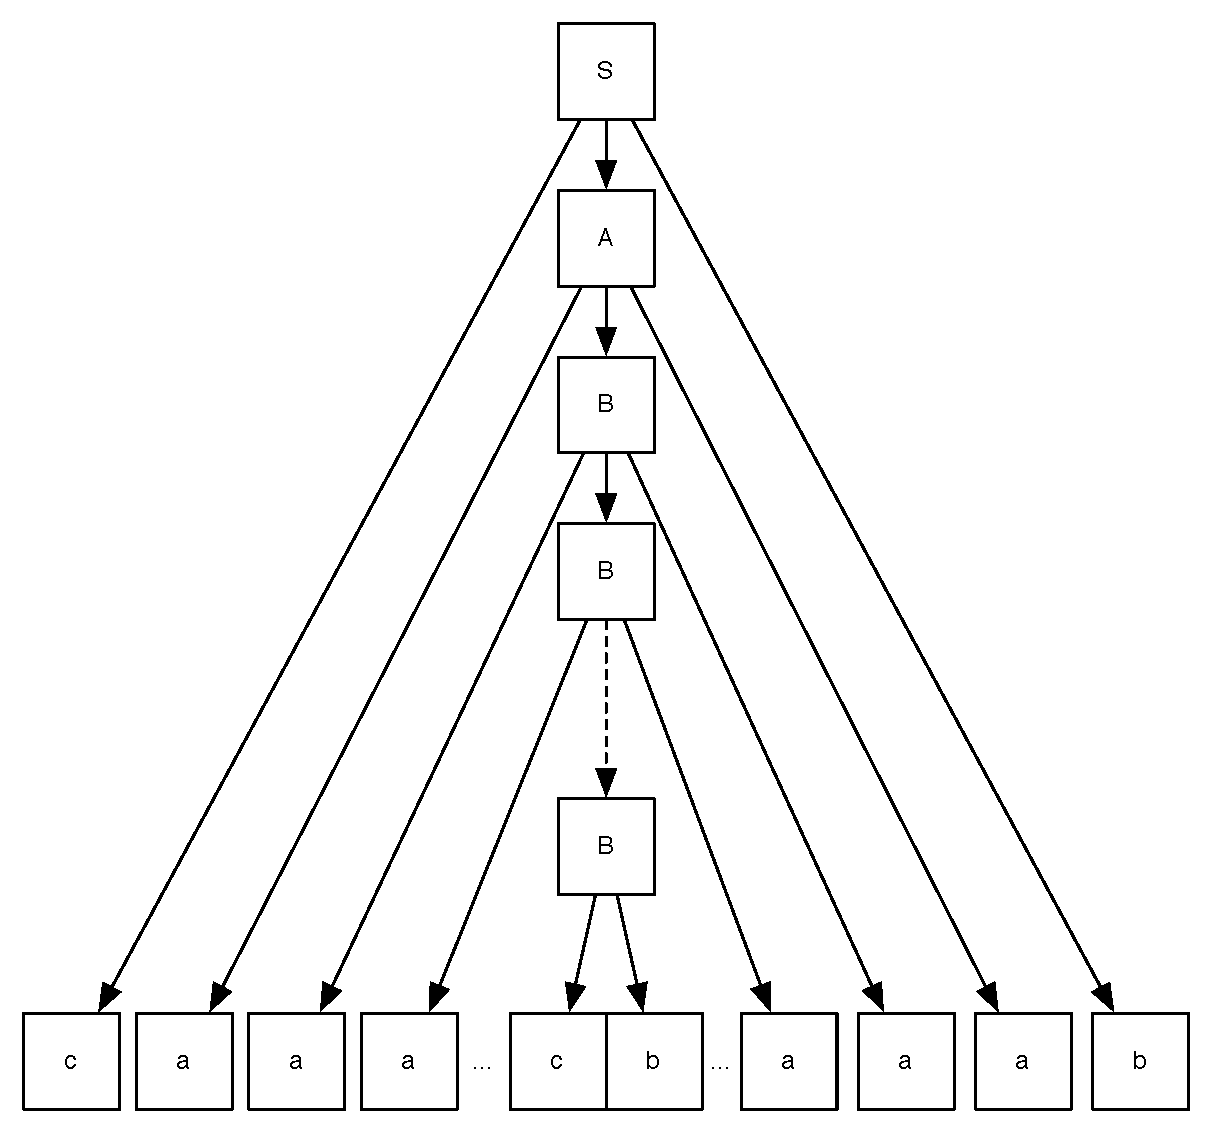
\includegraphics[width=15cm]{figures/grammar_abc}
\end{center}
	\caption{Arbre de d�rivation de la grammaire G}
	\label{grammar_abc}
\end{figure}\subsection{Arbres de d�rivation}

\section{Palindromes}

\subsection{Grammaire}
\begin{verbatim}
W := aWa | bWb | cWc | dWd | eWe | fWf | gWg | hWh | iWi | jWj | kWk | lWl | mWm | nWn 
W := oWo | pWp | qWq | rWr | sWs | tWt | uWu | vWv | wWw | xWx | yWy | zWz | 
W := a | b | c | d | e | f | g | h | i | j | k | l | m | n 
W := o | p | q | r | s | t | u | v | w | x | y | z | 
W := epsilon
\end{verbatim}

Cette grammaire est une grammaire alg�brique.

\subsection{Arbres de d�rivation}

\begin{figure}[!h]
\begin{center}
     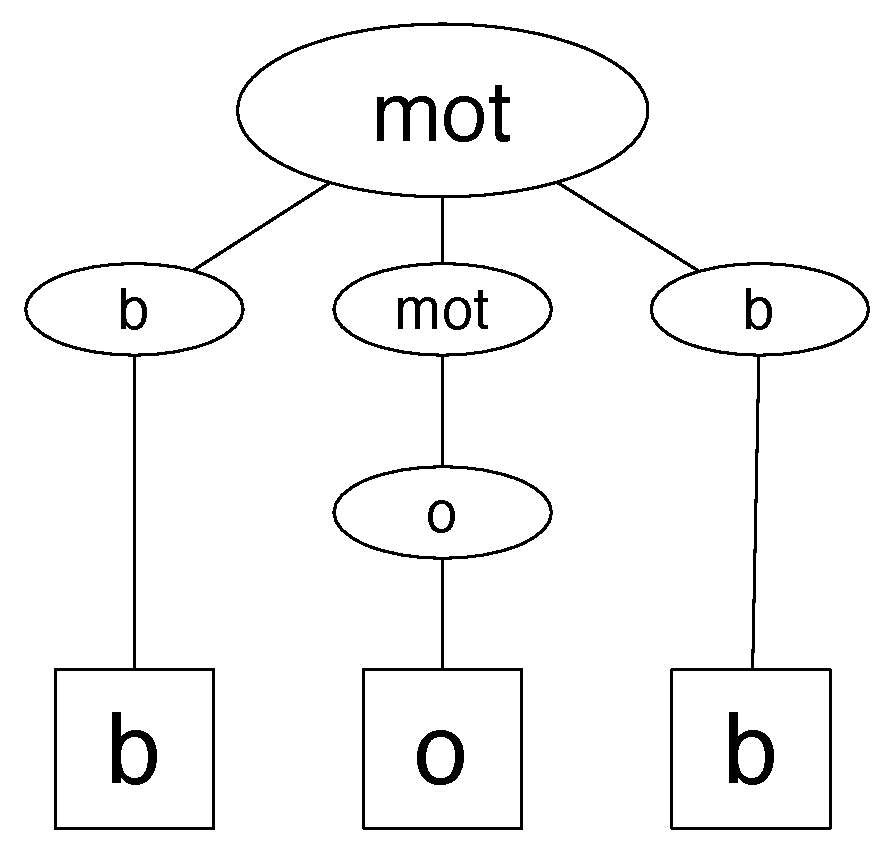
\includegraphics[width=6cm]{figures/derivation_bob}
\end{center}
     \caption{D�rivation du mot 'bob'}
\end{figure}

\begin{figure}[!h]
\begin{center}
     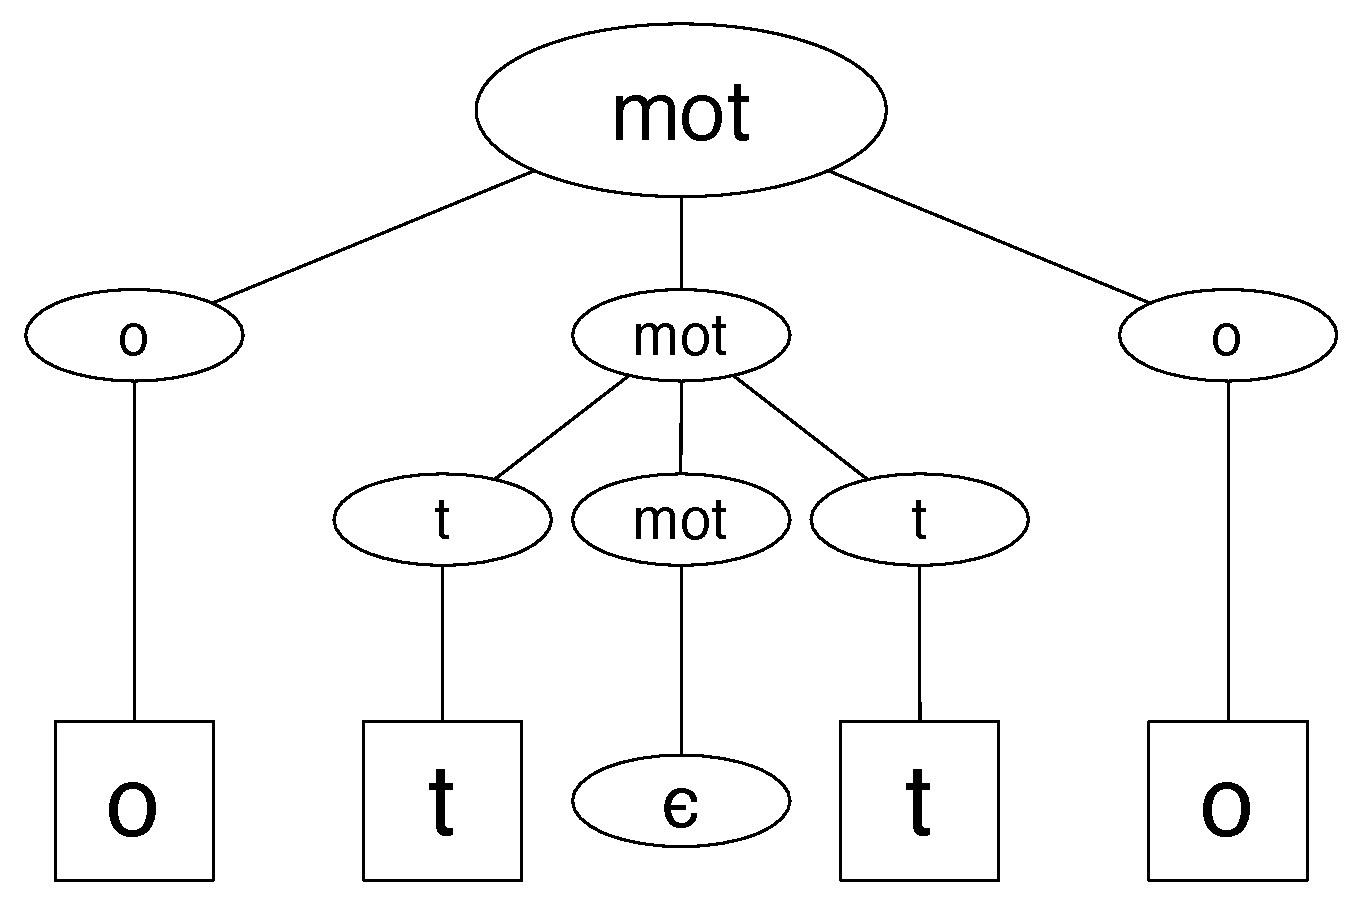
\includegraphics[width=8cm]{figures/derivation_otto}
\end{center}
     \caption{D�rivation du mot 'otto'}
\end{figure}

\newpage
\subsection{Impl�mentation en \pl}
Nous avons deux impl�mentations  en \pl, l'une bas�e sur l'inversion d'atome, l'autre sur l'extraction de sous atomes.


\begin{verbatimtab}
atom_reverse(X,X) :- atom_length(X,0).
atom_reverse(X,X) :- atom_length(X,1).
atom_reverse(X,Y) :- 
	atom_concat(A,B,X), 
	atom_length(A,1), 
	atom_reverse(B,B2), 
	atom_concat(B2, A,Y).

palindrome(X) :- atom_reverse(X, X).
\end{verbatimtab}


\begin{verbatimtab}
palindrome2(X) :- atom_length(X,0).
palindrome2(X) :- atom_length(X,1).
palindrome2(X) :- 
	atom_length(X,S), 
	P is S-1, 
	L is P-1, 
	sub_atom(X,0,1,_,A), 
	sub_atom(X,P,1,_,A), 
	sub_atom(X,1,L,_,W), 
	palindrome2(W).
\end{verbatimtab}


\end{document}